% !TEX encoding = UTF-8 Unicode
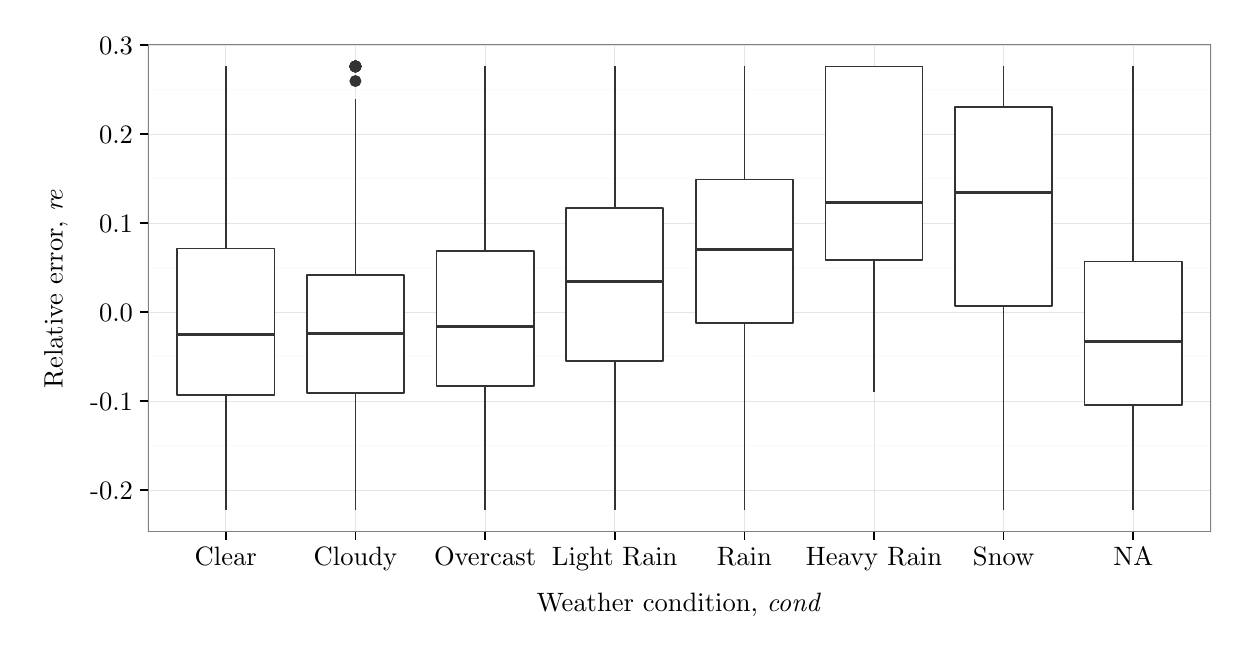
\begin{tikzpicture}[x=1pt,y=1pt]
\definecolor{fillColor}{RGB}{255,255,255}
\path[use as bounding box,fill=fillColor,fill opacity=0.00] (0,0) rectangle (433.62,216.81);
\begin{scope}
\path[clip] (  0.00,  0.00) rectangle (433.62,216.81);
\definecolor{drawColor}{RGB}{255,255,255}
\definecolor{fillColor}{RGB}{255,255,255}

\path[draw=drawColor,line width= 0.6pt,line join=round,line cap=round,fill=fillColor] (  0.00,  0.00) rectangle (433.62,216.81);
\end{scope}
\begin{scope}
\path[clip] ( 43.47, 34.62) rectangle (427.62,210.81);
\definecolor{fillColor}{RGB}{255,255,255}

\path[fill=fillColor] ( 43.47, 34.62) rectangle (427.62,210.81);
\definecolor{drawColor}{gray}{0.98}

\path[draw=drawColor,line width= 0.6pt,line join=round] ( 43.47, 65.84) --
	(427.62, 65.84);

\path[draw=drawColor,line width= 0.6pt,line join=round] ( 43.47, 98.00) --
	(427.62, 98.00);

\path[draw=drawColor,line width= 0.6pt,line join=round] ( 43.47,130.17) --
	(427.62,130.17);

\path[draw=drawColor,line width= 0.6pt,line join=round] ( 43.47,162.33) --
	(427.62,162.33);

\path[draw=drawColor,line width= 0.6pt,line join=round] ( 43.47,194.49) --
	(427.62,194.49);
\definecolor{drawColor}{gray}{0.90}

\path[draw=drawColor,line width= 0.2pt,line join=round] ( 43.47, 49.76) --
	(427.62, 49.76);

\path[draw=drawColor,line width= 0.2pt,line join=round] ( 43.47, 81.92) --
	(427.62, 81.92);

\path[draw=drawColor,line width= 0.2pt,line join=round] ( 43.47,114.08) --
	(427.62,114.08);

\path[draw=drawColor,line width= 0.2pt,line join=round] ( 43.47,146.25) --
	(427.62,146.25);

\path[draw=drawColor,line width= 0.2pt,line join=round] ( 43.47,178.41) --
	(427.62,178.41);

\path[draw=drawColor,line width= 0.2pt,line join=round] ( 43.47,210.57) --
	(427.62,210.57);

\path[draw=drawColor,line width= 0.2pt,line join=round] ( 71.58, 34.62) --
	( 71.58,210.81);

\path[draw=drawColor,line width= 0.2pt,line join=round] (118.43, 34.62) --
	(118.43,210.81);

\path[draw=drawColor,line width= 0.2pt,line join=round] (165.28, 34.62) --
	(165.28,210.81);

\path[draw=drawColor,line width= 0.2pt,line join=round] (212.12, 34.62) --
	(212.12,210.81);

\path[draw=drawColor,line width= 0.2pt,line join=round] (258.97, 34.62) --
	(258.97,210.81);

\path[draw=drawColor,line width= 0.2pt,line join=round] (305.82, 34.62) --
	(305.82,210.81);

\path[draw=drawColor,line width= 0.2pt,line join=round] (352.66, 34.62) --
	(352.66,210.81);

\path[draw=drawColor,line width= 0.2pt,line join=round] (399.51, 34.62) --
	(399.51,210.81);
\definecolor{drawColor}{gray}{0.20}

\path[draw=drawColor,line width= 0.6pt,line join=round] ( 71.58,136.97) -- ( 71.58,202.80);

\path[draw=drawColor,line width= 0.6pt,line join=round] ( 71.58, 84.19) -- ( 71.58, 42.63);

\path[draw=drawColor,line width= 0.6pt,line join=round,line cap=round,fill=fillColor] ( 54.02,136.97) --
	( 54.02, 84.19) --
	( 89.15, 84.19) --
	( 89.15,136.97) --
	( 54.02,136.97) --
	cycle;

\path[draw=drawColor,line width= 1.1pt,line join=round] ( 54.02,105.90) -- ( 89.15,105.90);
\definecolor{fillColor}{gray}{0.20}

\path[draw=drawColor,line width= 0.4pt,line join=round,line cap=round,fill=fillColor] (118.43,202.80) circle (  1.96);

\path[draw=drawColor,line width= 0.4pt,line join=round,line cap=round,fill=fillColor] (118.43,202.80) circle (  1.96);

\path[draw=drawColor,line width= 0.4pt,line join=round,line cap=round,fill=fillColor] (118.43,202.80) circle (  1.96);

\path[draw=drawColor,line width= 0.4pt,line join=round,line cap=round,fill=fillColor] (118.43,202.80) circle (  1.96);

\path[draw=drawColor,line width= 0.4pt,line join=round,line cap=round,fill=fillColor] (118.43,197.52) circle (  1.96);

\path[draw=drawColor,line width= 0.4pt,line join=round,line cap=round,fill=fillColor] (118.43,202.80) circle (  1.96);

\path[draw=drawColor,line width= 0.4pt,line join=round,line cap=round,fill=fillColor] (118.43,202.80) circle (  1.96);

\path[draw=drawColor,line width= 0.4pt,line join=round,line cap=round,fill=fillColor] (118.43,202.80) circle (  1.96);

\path[draw=drawColor,line width= 0.4pt,line join=round,line cap=round,fill=fillColor] (118.43,202.80) circle (  1.96);

\path[draw=drawColor,line width= 0.4pt,line join=round,line cap=round,fill=fillColor] (118.43,202.80) circle (  1.96);

\path[draw=drawColor,line width= 0.4pt,line join=round,line cap=round,fill=fillColor] (118.43,202.80) circle (  1.96);

\path[draw=drawColor,line width= 0.6pt,line join=round] (118.43,127.44) -- (118.43,191.09);

\path[draw=drawColor,line width= 0.6pt,line join=round] (118.43, 84.77) -- (118.43, 42.63);
\definecolor{fillColor}{RGB}{255,255,255}

\path[draw=drawColor,line width= 0.6pt,line join=round,line cap=round,fill=fillColor] (100.86,127.44) --
	(100.86, 84.77) --
	(136.00, 84.77) --
	(136.00,127.44) --
	(100.86,127.44) --
	cycle;

\path[draw=drawColor,line width= 1.1pt,line join=round] (100.86,106.45) -- (136.00,106.45);

\path[draw=drawColor,line width= 0.6pt,line join=round] (165.28,136.11) -- (165.28,202.80);

\path[draw=drawColor,line width= 0.6pt,line join=round] (165.28, 87.40) -- (165.28, 42.63);

\path[draw=drawColor,line width= 0.6pt,line join=round,line cap=round,fill=fillColor] (147.71,136.11) --
	(147.71, 87.40) --
	(182.84, 87.40) --
	(182.84,136.11) --
	(147.71,136.11) --
	cycle;

\path[draw=drawColor,line width= 1.1pt,line join=round] (147.71,108.82) -- (182.84,108.82);

\path[draw=drawColor,line width= 0.6pt,line join=round] (212.12,151.69) -- (212.12,202.80);

\path[draw=drawColor,line width= 0.6pt,line join=round] (212.12, 96.43) -- (212.12, 42.63);

\path[draw=drawColor,line width= 0.6pt,line join=round,line cap=round,fill=fillColor] (194.56,151.69) --
	(194.56, 96.43) --
	(229.69, 96.43) --
	(229.69,151.69) --
	(194.56,151.69) --
	cycle;

\path[draw=drawColor,line width= 1.1pt,line join=round] (194.56,125.17) -- (229.69,125.17);

\path[draw=drawColor,line width= 0.6pt,line join=round] (258.97,161.90) -- (258.97,202.80);

\path[draw=drawColor,line width= 0.6pt,line join=round] (258.97,110.03) -- (258.97, 42.63);

\path[draw=drawColor,line width= 0.6pt,line join=round,line cap=round,fill=fillColor] (241.40,161.90) --
	(241.40,110.03) --
	(276.54,110.03) --
	(276.54,161.90) --
	(241.40,161.90) --
	cycle;

\path[draw=drawColor,line width= 1.1pt,line join=round] (241.40,136.63) -- (276.54,136.63);

\path[draw=drawColor,line width= 0.6pt,line join=round] (305.82,202.80) -- (305.82,202.80);

\path[draw=drawColor,line width= 0.6pt,line join=round] (305.82,132.86) -- (305.82, 85.09);

\path[draw=drawColor,line width= 0.6pt,line join=round,line cap=round,fill=fillColor] (288.25,202.80) --
	(288.25,132.86) --
	(323.39,132.86) --
	(323.39,202.80) --
	(288.25,202.80) --
	cycle;

\path[draw=drawColor,line width= 1.1pt,line join=round] (288.25,153.56) -- (323.39,153.56);

\path[draw=drawColor,line width= 0.6pt,line join=round] (352.66,188.15) -- (352.66,202.80);

\path[draw=drawColor,line width= 0.6pt,line join=round] (352.66,116.22) -- (352.66, 42.63);

\path[draw=drawColor,line width= 0.6pt,line join=round,line cap=round,fill=fillColor] (335.10,188.15) --
	(335.10,116.22) --
	(370.23,116.22) --
	(370.23,188.15) --
	(335.10,188.15) --
	cycle;

\path[draw=drawColor,line width= 1.1pt,line join=round] (335.10,157.13) -- (370.23,157.13);

\path[draw=drawColor,line width= 0.6pt,line join=round] (399.51,132.34) -- (399.51,202.80);

\path[draw=drawColor,line width= 0.6pt,line join=round] (399.51, 80.57) -- (399.51, 42.63);

\path[draw=drawColor,line width= 0.6pt,line join=round,line cap=round,fill=fillColor] (381.94,132.34) --
	(381.94, 80.57) --
	(417.08, 80.57) --
	(417.08,132.34) --
	(381.94,132.34) --
	cycle;

\path[draw=drawColor,line width= 1.1pt,line join=round] (381.94,103.38) -- (417.08,103.38);
\definecolor{drawColor}{gray}{0.50}

\path[draw=drawColor,line width= 0.6pt,line join=round,line cap=round] ( 43.47, 34.62) rectangle (427.62,210.81);
\end{scope}
\begin{scope}
\path[clip] (  0.00,  0.00) rectangle (433.62,216.81);
\definecolor{drawColor}{RGB}{0,0,0}

\node[text=drawColor,anchor=base east,inner sep=0pt, outer sep=0pt, scale=  0.96] at ( 38.07, 46.45) {-0.2};

\node[text=drawColor,anchor=base east,inner sep=0pt, outer sep=0pt, scale=  0.96] at ( 38.07, 78.62) {-0.1};

\node[text=drawColor,anchor=base east,inner sep=0pt, outer sep=0pt, scale=  0.96] at ( 38.07,110.78) {0.0};

\node[text=drawColor,anchor=base east,inner sep=0pt, outer sep=0pt, scale=  0.96] at ( 38.07,142.94) {0.1};

\node[text=drawColor,anchor=base east,inner sep=0pt, outer sep=0pt, scale=  0.96] at ( 38.07,175.10) {0.2};

\node[text=drawColor,anchor=base east,inner sep=0pt, outer sep=0pt, scale=  0.96] at ( 38.07,207.27) {0.3};
\end{scope}
\begin{scope}
\path[clip] (  0.00,  0.00) rectangle (433.62,216.81);
\definecolor{drawColor}{RGB}{0,0,0}

\path[draw=drawColor,line width= 0.6pt,line join=round] ( 40.47, 49.76) --
	( 43.47, 49.76);

\path[draw=drawColor,line width= 0.6pt,line join=round] ( 40.47, 81.92) --
	( 43.47, 81.92);

\path[draw=drawColor,line width= 0.6pt,line join=round] ( 40.47,114.08) --
	( 43.47,114.08);

\path[draw=drawColor,line width= 0.6pt,line join=round] ( 40.47,146.25) --
	( 43.47,146.25);

\path[draw=drawColor,line width= 0.6pt,line join=round] ( 40.47,178.41) --
	( 43.47,178.41);

\path[draw=drawColor,line width= 0.6pt,line join=round] ( 40.47,210.57) --
	( 43.47,210.57);
\end{scope}
\begin{scope}
\path[clip] (  0.00,  0.00) rectangle (433.62,216.81);
\definecolor{drawColor}{RGB}{0,0,0}

\path[draw=drawColor,line width= 0.6pt,line join=round] ( 71.58, 31.62) --
	( 71.58, 34.62);

\path[draw=drawColor,line width= 0.6pt,line join=round] (118.43, 31.62) --
	(118.43, 34.62);

\path[draw=drawColor,line width= 0.6pt,line join=round] (165.28, 31.62) --
	(165.28, 34.62);

\path[draw=drawColor,line width= 0.6pt,line join=round] (212.12, 31.62) --
	(212.12, 34.62);

\path[draw=drawColor,line width= 0.6pt,line join=round] (258.97, 31.62) --
	(258.97, 34.62);

\path[draw=drawColor,line width= 0.6pt,line join=round] (305.82, 31.62) --
	(305.82, 34.62);

\path[draw=drawColor,line width= 0.6pt,line join=round] (352.66, 31.62) --
	(352.66, 34.62);

\path[draw=drawColor,line width= 0.6pt,line join=round] (399.51, 31.62) --
	(399.51, 34.62);
\end{scope}
\begin{scope}
\path[clip] (  0.00,  0.00) rectangle (433.62,216.81);
\definecolor{drawColor}{RGB}{0,0,0}

\node[text=drawColor,anchor=base,inner sep=0pt, outer sep=0pt, scale=  0.96] at ( 71.58, 22.61) {Clear};

\node[text=drawColor,anchor=base,inner sep=0pt, outer sep=0pt, scale=  0.96] at (118.43, 22.61) {Cloudy};

\node[text=drawColor,anchor=base,inner sep=0pt, outer sep=0pt, scale=  0.96] at (165.28, 22.61) {Overcast};

\node[text=drawColor,anchor=base,inner sep=0pt, outer sep=0pt, scale=  0.96] at (212.12, 22.61) {Light Rain};

\node[text=drawColor,anchor=base,inner sep=0pt, outer sep=0pt, scale=  0.96] at (258.97, 22.61) {Rain};

\node[text=drawColor,anchor=base,inner sep=0pt, outer sep=0pt, scale=  0.96] at (305.82, 22.61) {Heavy Rain};

\node[text=drawColor,anchor=base,inner sep=0pt, outer sep=0pt, scale=  0.96] at (352.66, 22.61) {Snow};

\node[text=drawColor,anchor=base,inner sep=0pt, outer sep=0pt, scale=  0.96] at (399.51, 22.61) {NA};
\end{scope}
\begin{scope}
\path[clip] (  0.00,  0.00) rectangle (433.62,216.81);
\definecolor{drawColor}{RGB}{0,0,0}

\node[text=drawColor,anchor=base,inner sep=0pt, outer sep=0pt, scale=  0.96] at (235.55,  6.00) {Weather condition, $\mathit{cond}$};
\end{scope}
\begin{scope}
\path[clip] (  0.00,  0.00) rectangle (433.62,216.81);
\definecolor{drawColor}{RGB}{0,0,0}

\node[text=drawColor,rotate= 90.00,anchor=base,inner sep=0pt, outer sep=0pt, scale=  0.96] at ( 12.61,122.72) {Relative error, $\mathit{re}$};
\end{scope}
\end{tikzpicture}
